\documentclass[10pt]{article}

\usepackage{amsmath}
\usepackage{amsfonts}
\usepackage{graphicx}

\begin{document} 
\title{Resumen de Analisis Numerico}
\author{
        Mateo P. Cetti \\
        Estudiante - Universdad Catolica de Cordoba\\
        Ing Ambrosio Taravella, 6240, \underline{Cordoba, Argentina}
}
\date{\today}

\maketitle

\section{Introduccion}

\subsection{Objetivo del analisis numerico}

El objetivo del analisis numerico es el de enseñarle 
a la computadora a realizar operaciones matematicas complejas.
Se estudian metodos numericos que nos permiten interactuar con la computadora

Antiguamente los metodos numericos eran usados de manera muy limitada por el 
tedioso trabajo de usarlos a mano. Ahora con el auge de las computadoras, 
estos modelos son mas usados y generan mucho mejores resultados.

\subsection{Problematicas}

\begin{enumerate}
	\item Las computadoras no trabajan en un universo \textbf{infinito} (Ojo con el acarreo del error). En nuestra mente
	hay infinitos numeros, y entre dos numeros tambien hay infinitos numeros (Universo discreto y acotado).
	\item Las computadoras trabajan internamente con el sistema \textbf{binario}, y los numeros
	tienen un espacio "finito" de digitos. Utilizan la notacion de \textbf{mantisa} y \textbf{exponente}.
	\item Como en el desarrollo de Taylor, los metodos numericos se basan en formulaciones 
	teoricas \textbf{complejas} e \textbf{infinitas}.
\end{enumerate}

\pagebreak

\section{Conceptos elementales}

\begin{itemize}
	\item \textbf{Digitio}: Unidad elemental en la representacion de un numero.
	\item \textbf{Numero}: Conjunto de digitos que conforman un elemento.
	\item \textbf{Cifras}: Cantidad de digitos.
	\item \textbf{Cifras significativas}: Cantidad de digitos que poseen un valor confiable.
	\item \textbf{Error}: Diferencia entre valor real y un valor proximo al real.
	\item \textbf{Exactitud}:Aproximacion de un numero a su valor verdadero.
	\item \textbf{Precisión}: Esta relacionada al grado de \textbf{dispersión} 
	entre los \textbf{valores aproximados}.
	
	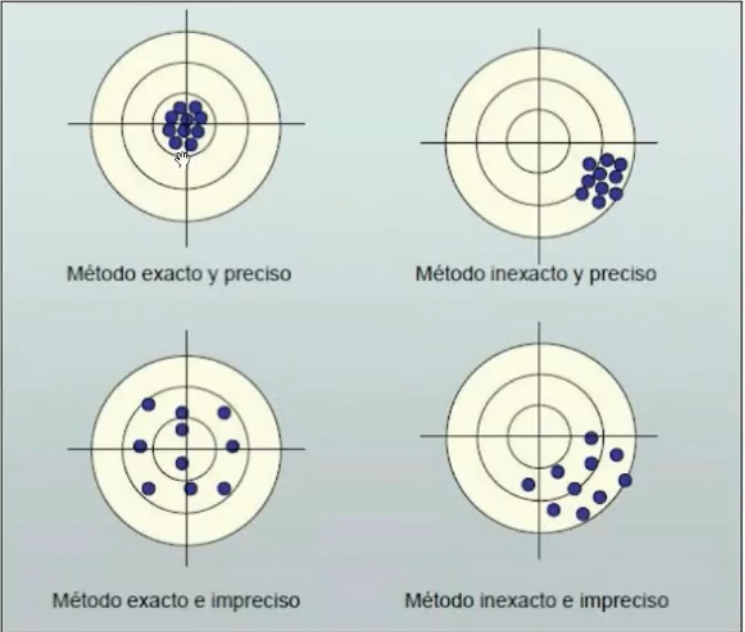
\includegraphics[width = 200px]{./img/tiro_al_blanco.png}
\end{itemize}

\subsection{Errores}

Valor aproximado entre un valor \textbf{real} y uno \textbf{proximo}.

\begin{equation}
	E = x_v - x_a
\end{equation}

Esto (1) se conoce como \textbf{error total}. En muchas ocaciones se trabaja
con el \textbf{error relativo} (2):

\begin{equation}
	E_r = \dfrac{x_v - x_a}{x_v}
\end{equation}

Y muchas otras veces se utiliza el \textbf{error relativo porcentual} (3):

\begin{equation}
	E_r = \dfrac{x_v - x_a}{x_v} 100%
\end{equation}

Muchos de los metodos son iterativos (Mejoran los resultados en cada iteracion). 
En la practica el valor \textbf{verdadero} no se conoce, por lo que se suele
trabajar con \textbf{errores aproximados} o aproximacion de errores.

\begin{equation}
	E_a = x_{actual} - x_{previo}
\end{equation}

\begin{equation}
	E_{ra} = \dfrac{x_{actual} - x_{previo}}{x_{actual}}
\end{equation}

\begin{equation}
	E_{ra}[\%] = \dfrac{x_{actual} - x_{previo}}{x_{actual}}100
\end{equation}

Si dichos errores aumentan con cada iteracion decimos que el metodo 
\textbf{diverge} a la solucion (El metodo no sirve para el problema elegido).
Sino, decimos que el metodo \textbf{converge} en la solucion

\pagebreak

\section{Raices de ecuaciones lineales}

\subsection{Presentacion del problema}

Para diversos problemas (Ej: amortiguacion de un auto) es muy utiliza
averiguar raices de ecuaciones.

\subsection{Metodo de la biseccion}

Este metodo sirve para todas las funciones excepto aquellas que tengan
\textbf{raices multiples de orden par}. Este metodo consiste en elegir 
\textbf{dos puntos} en una funcion continua y multiplicarlos Si hay un 
cambio de signo entonces en el intervalo entre ambos puntos 
\textbf{hay una raiz} (o mas de una).

\begin{equation}
	f(a)f(b) \leq 0
\end{equation}

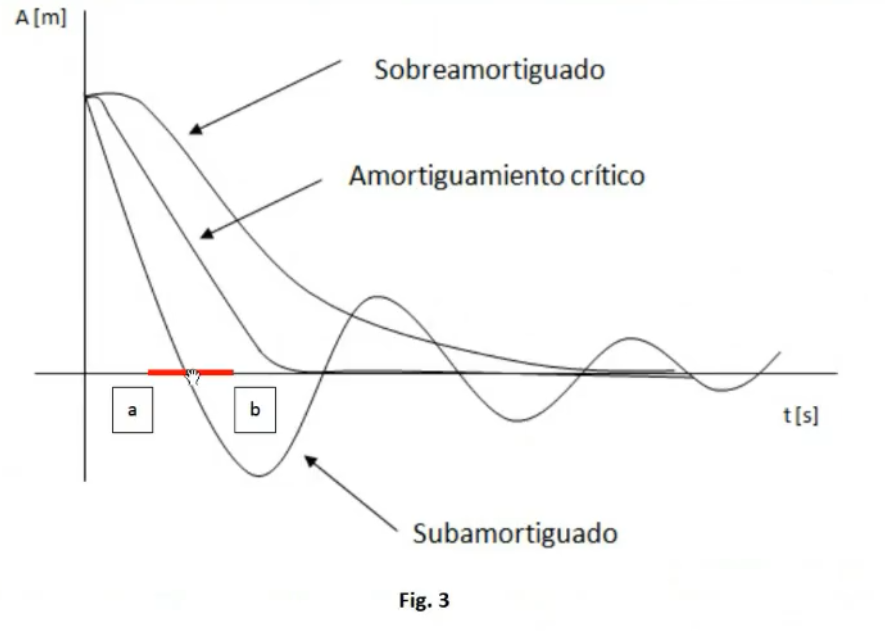
\includegraphics[width = 300px]{./img/biseccion.png}

Este metodo \textbf{no es util} cuando hay \textbf{muchas raices} 
en \textbf{intervalos muy pequeños}, ya que no nos dice la 
cantidad exacta de raices en el intervalo elegido.

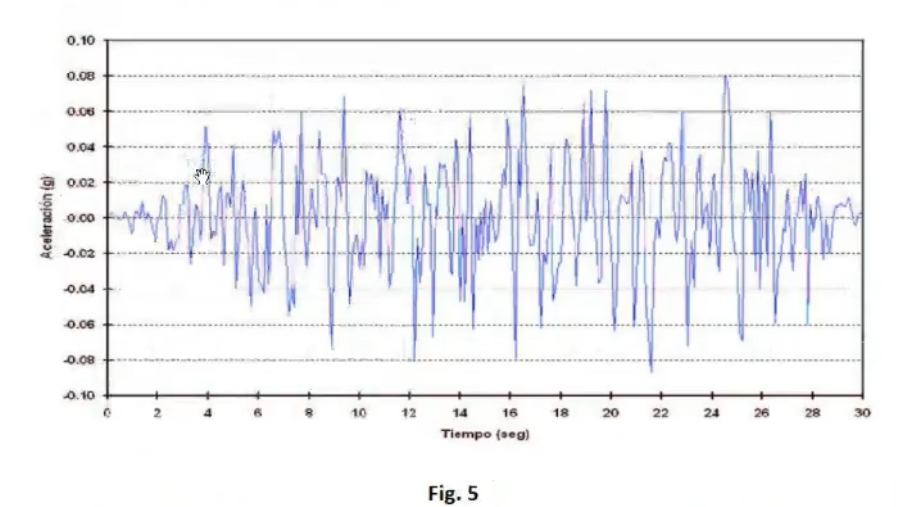
\includegraphics[width = 300px]{./img/sismo.png}

Para \textbf{calcular} la raiz de una funcion, se eligen los puntos
$a$ y $b$ y se aplica el metodo. Si hay una raiz, entonces se vuelve
a realizar el metodo pero en el intervalo $a$ y $c$ o $c$ y $a$ en 
donde c es:

\begin{equation}
	c = \dfrac{a+b}{2}
\end{equation}

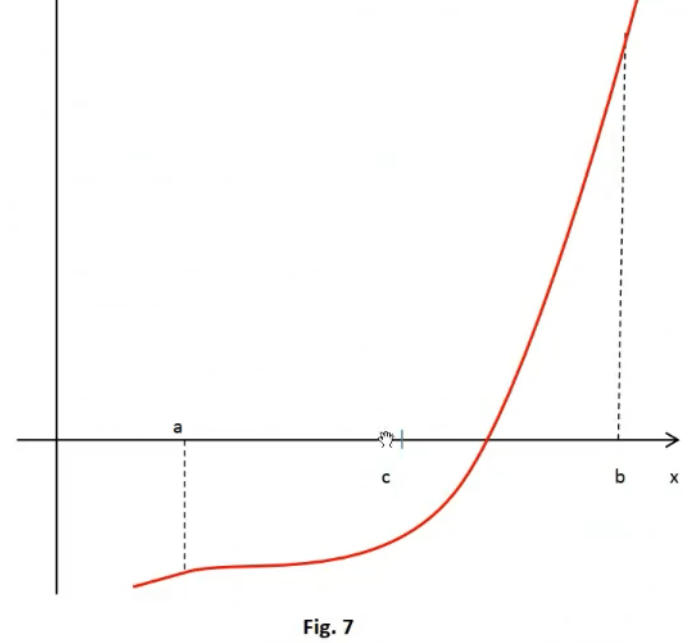
\includegraphics[width = 300px]{./img/biseccion_calcular.png}

Si $f(a)f(c) \leq 0$ entonces la raiz esta en el intervalo $a$ y 
$c$. sino, esta en el intervalo $c$ y $b$ 

\textbf{Ventajas de este metodo}

\begin{itemize}
	\item Alto grado de convergencia
	\item Confiable
	\item Facil programacion
\end{itemize}

\textbf{Desventajas}

\begin{itemize}
	\item No es apto para raices multiples de orden par
	\item convergencia \textbf{lenta}
\end{itemize}

\subsection{Metodo de punto fijo}

Este metodo coinciste en generar una funcion $g(x)$ a partir de la
funcion $f(x)$ original que intersecte a la funcion identidad.
De ser ese el caso, llamamos al punto interseccion punto fijo,
y en su dominio encontraremos la raiz de la funcion original.

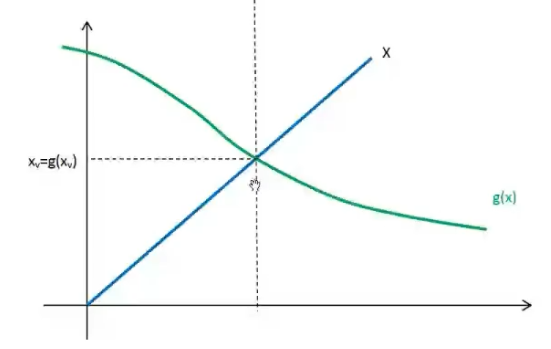
\includegraphics[width = 300px]{./img/punto_fijo.png}

\begin{equation}
	x_v = g(x_v)
\end{equation}

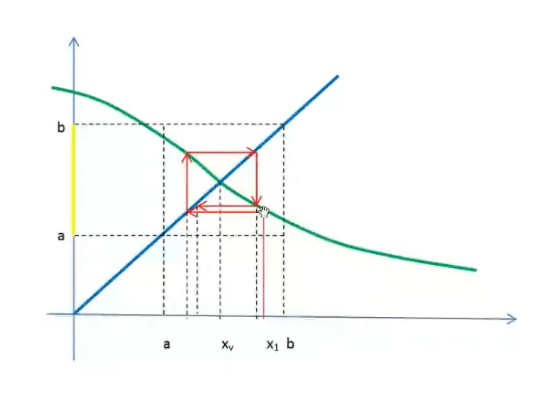
\includegraphics[width = 300px]{./img/punto_fijo_2.png}

Estas funciones $g(x)$ se obtienen de la funcion $f(x)$ original
de varias formas:

\begin{itemize}
	\item Por simple despeje
	\item Sumando o restando a ambos lados $x$ 
	\item Utilizando algun otro metodo matematico
	\item Proponiendo una $g(x)$ (Solo si se esta muy canchero)
\end{itemize}

No todas las funciones $g(x)$ funcionan, cuando no funcionan decimos
que son funciones \textbf{divergentes}. Para asegurarnos que la funcion
se comporte de manera \textbf{convergente}, esta debe cumplir con con 2 coindiciones:

\begin{enumerate}
	\item $g(x) \in [a, b]$ (amarillo)
	\item $|g'(\varepsilon)| \leq 1$ y $\varepsilon$ maximice la derivada
\end{enumerate}

Empezamos con $\varepsilon$ y aplicamos la formula:

\begin{equation}
	x_{i+1} = g(x_i)
\end{equation}

\textbf{Ventajas}

\begin{enumerate}
	\item Rapida convergencia
	\item Facil de programar
	\item Se puede partir de un valor proxmio sin importar de que lado esta la raiz (Metodo abierto)
\end{enumerate}

\textbf{Desventajas}

\begin{enumerate}
	\item Dificultad para encontrar una $g(x)$ convergente
	\item Puede quedar en un \textbf{lazo anidado}
\end{enumerate}

\end{document}